
\thispagestyle{empty}
%\put(0,0){
\begin{minipage}[h]{0.9\paperwidth}
\thispagestyle{empty}
\begin{tikzpicture}[remember picture,overlay]
\node (f) [rectangle]  
at (current page.center)
          {\parbox[b][\paperheight]{\paperwidth}{
           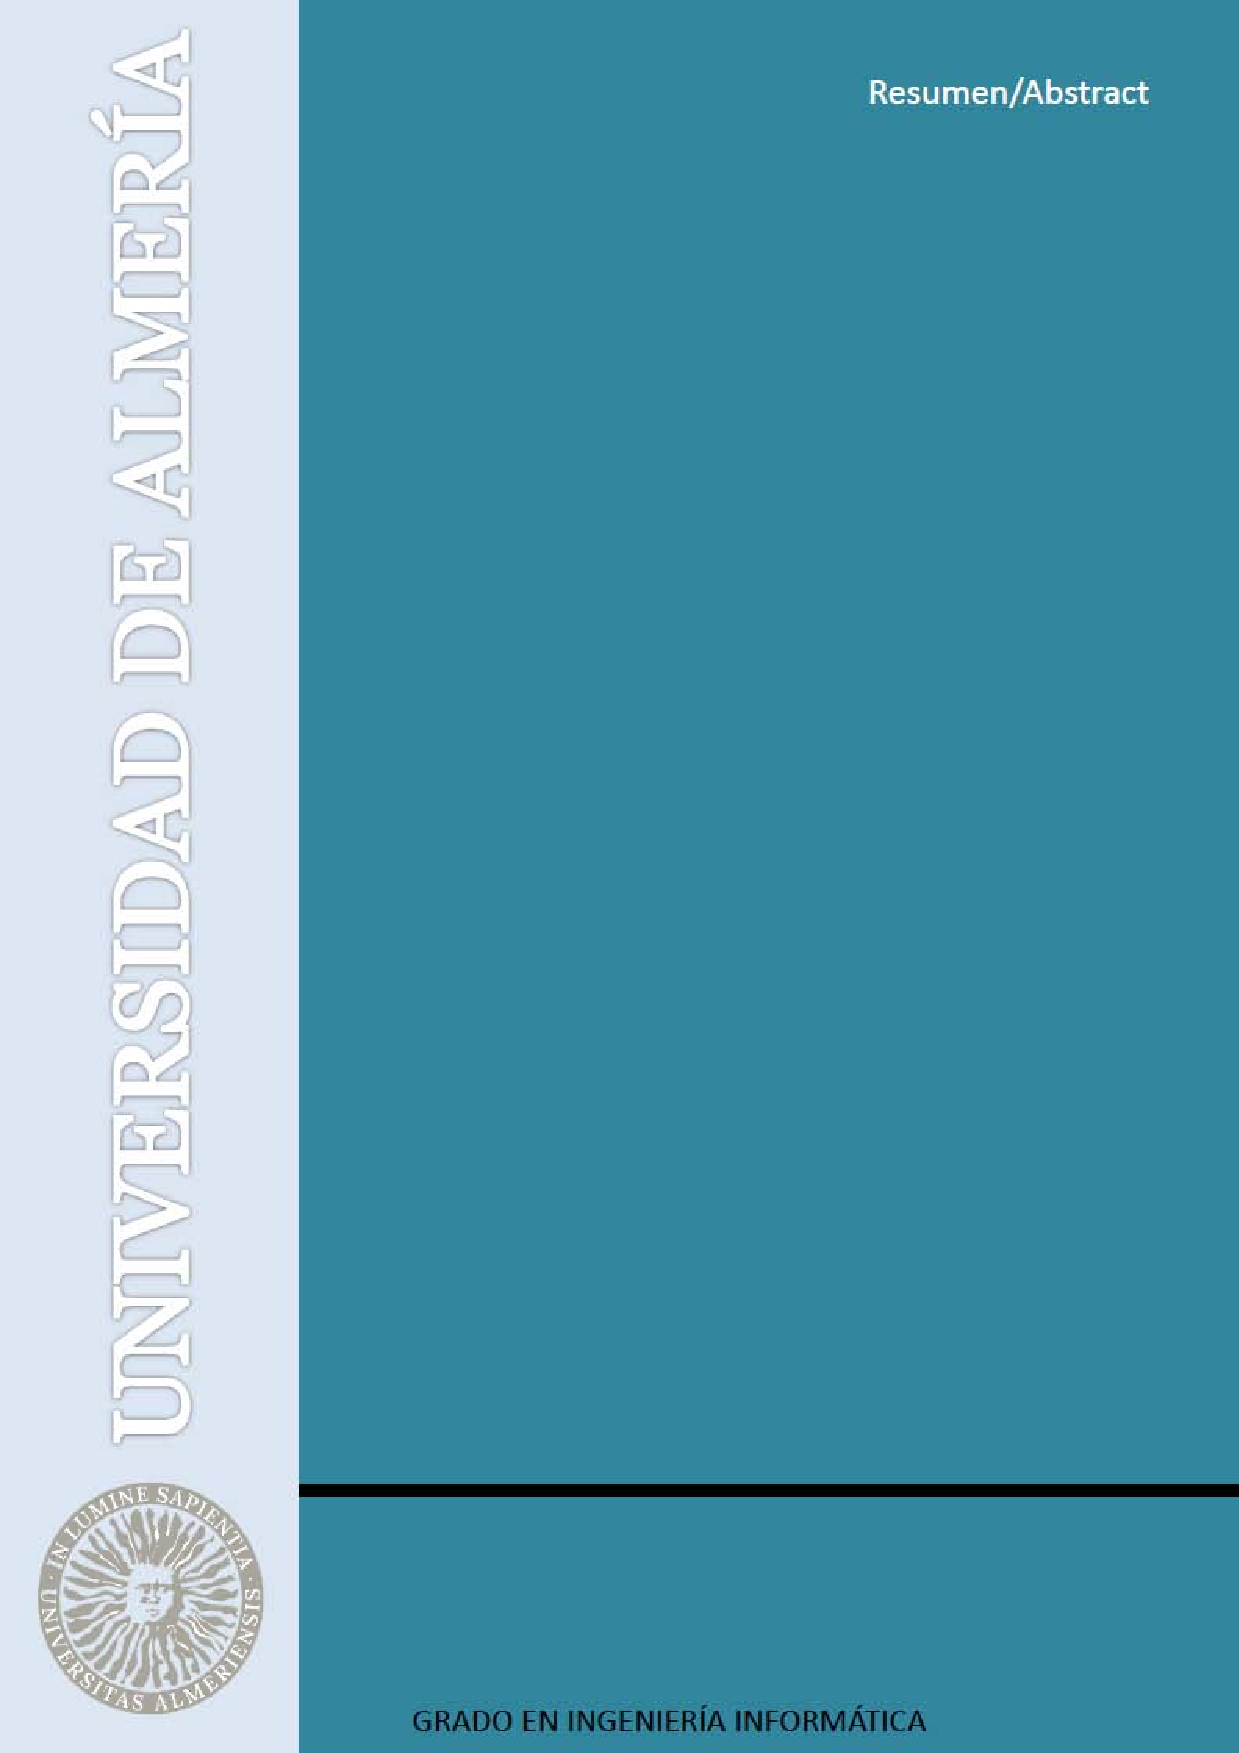
\includegraphics[width=\paperwidth,height=\paperheight,keepaspectratio]{Figuras/logos/TFG_back}
          }};
\node (texto) [rectangle,text width=0.5\paperwidth,yshift=150pt] 
at (f)
          %{\parbox{0.65\paperwidth}{\justifying \Large \color{white}
          {\parbox{0.65\paperwidth}{\justifying \color{white}
         En este archivo se incluirá tanto el resumen en castellano como su traducción al inglés. Los dos párrafos estarán ligeramente separados.

El  propósito  del  trabajo  en  una  o  dos  frases.  El  diseño  y metodología  utilizada,  los  resultados  más  significativos  del trabajo realizado y un breve resumen de las conclusiones. Debe ser conciso y presentar los resultados obtenidos tras la ejecución del TFG. 

\vspace{1.5cm}

%\section*{Abstract}
Put here  the english translation  ... . Debe ser conciso y presentar los resultados obtenidos tras la ejecución del TFG. Los dos parrafos estarán ligeramente separados.
         }};
       \node  at (14,-25.55) {\Large\curso};
  \end{tikzpicture}
\end{minipage}
%}


          
          